\documentclass{article}
\usepackage{amsmath}
\usepackage{amssymb}
\usepackage{graphicx}
\usepackage{hyperref}
\usepackage[version=4]{mhchem}

\title{Example 6}
\date{}

\begin{document}
\maketitle

In triangle \(A B C\), a point \(D\) is taken on \(A B\) and a point \(E\) is taken on \(A C\) such that \(B D: D C=3: 2\), and \(A E: E C=3: 4 . A D\) and \(B E\) intersect at \(M\). Find the area of triangle \(B M D\) if the area of triangle \(A B C\) is 1 .

Solution: \(\frac{4}{15}\).\\
\centering
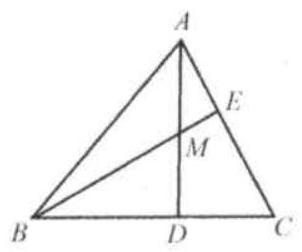
\includegraphics[width=\textwidth]{images/problem_image_1.jpg}

Draw \(E N / / A D\) to meet \(B C\) at \(N\).\\
Since \(B D: D C=3: 2\) and \(A E: E C=3: 4, N C: D N: B D=8: 6\) \(: 21\).\\
We know that \(S_{\triangle B C E}=\frac{4}{7} S_{\triangle A B C}=\frac{4}{7}\). Thus\\
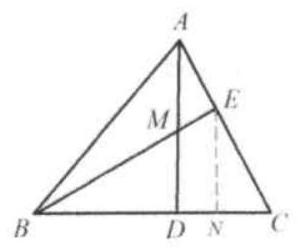
\includegraphics[width=\textwidth]{images/reasoning_image_1.jpg} \(S_{\triangle B N E}=\frac{27}{35} S_{\triangle B E C}=\frac{27 \times 4}{35 \times 7}\).\\
Since \(D M / / E N, \triangle B D M \sim \triangle B N E\). Then \(S_{A B D M}=\left(\frac{21}{27}\right)^{2} S_{A B N C}=\frac{49}{81} \times \frac{27 \times 4}{35 \times 7}=\frac{4}{15}\)\\

\end{document}
